% This is the Reed College LaTeX thesis template. Most of the work
% for the document class was done by Sam Noble (SN), as well as this
% template. Later comments etc. by Ben Salzberg (BTS). Additional
% restructuring and APA support by Jess Youngberg (JY).
% Your comments and suggestions are more than welcome; please email
% them to cus@reed.edu
%
% See https://www.reed.edu/cis/help/LaTeX/index.html for help. There are a
% great bunch of help pages there, with notes on
% getting started, bibtex, etc. Go there and read it if you're not
% already familiar with LaTeX.
%
% Any line that starts with a percent symbol is a comment.
% They won't show up in the document, and are useful for notes
% to yourself and explaining commands.
% Commenting also removes a line from the document;
% very handy for troubleshooting problems. -BTS

% As far as I know, this follows the requirements laid out in
% the 2002-2003 Senior Handbook. Ask a librarian to check the
% document before binding. -SN

%%
%% Preamble
%%
% \documentclass{<something>} must begin each LaTeX document
\documentclass[12pt,twoside]{reedthesis}
% Packages are extensions to the basic LaTeX functions. Whatever you
% want to typeset, there is probably a package out there for it.
% Chemistry (chemtex), screenplays, you name it.
% Check out CTAN to see: https://www.ctan.org/
%%
\usepackage{graphicx,latexsym}
\usepackage{amsmath}
\usepackage{amssymb,amsthm}
\usepackage{longtable,booktabs,setspace}
\usepackage{chemarr} %% Useful for one reaction arrow, useless if you're not a chem major
\usepackage[hyphens]{url}
% Added by CII
\usepackage{hyperref}
\usepackage{lmodern}
\usepackage{float}
\floatplacement{figure}{H}
% End of CII addition
\usepackage{rotating}

% Next line commented out by CII
%%% \usepackage{natbib}
% Comment out the natbib line above and uncomment the following two lines to use the new
% biblatex-chicago style, for Chicago A. Also make some changes at the end where the
% bibliography is included.
%\usepackage{biblatex-chicago}
%\bibliography{thesis}


% Added by CII (Thanks, Hadley!)
% Use ref for internal links
\renewcommand{\hyperref}[2][???]{\autoref{#1}}
\def\chapterautorefname{Chapter}
\def\sectionautorefname{Section}
\def\subsectionautorefname{Subsection}
% End of CII addition

% Added by CII
\usepackage{caption}
\captionsetup{width=5in}
% End of CII addition

% \usepackage{times} % other fonts are available like times, bookman, charter, palatino

% Syntax highlighting #22
  \usepackage{color}
  \usepackage{fancyvrb}
  \newcommand{\VerbBar}{|}
  \newcommand{\VERB}{\Verb[commandchars=\\\{\}]}
  \DefineVerbatimEnvironment{Highlighting}{Verbatim}{commandchars=\\\{\}}
  % Add ',fontsize=\small' for more characters per line
  \usepackage{framed}
  \definecolor{shadecolor}{RGB}{248,248,248}
  \newenvironment{Shaded}{\begin{snugshade}}{\end{snugshade}}
  \newcommand{\AlertTok}[1]{\textcolor[rgb]{0.94,0.16,0.16}{#1}}
  \newcommand{\AnnotationTok}[1]{\textcolor[rgb]{0.56,0.35,0.01}{\textbf{\textit{#1}}}}
  \newcommand{\AttributeTok}[1]{\textcolor[rgb]{0.77,0.63,0.00}{#1}}
  \newcommand{\BaseNTok}[1]{\textcolor[rgb]{0.00,0.00,0.81}{#1}}
  \newcommand{\BuiltInTok}[1]{#1}
  \newcommand{\CharTok}[1]{\textcolor[rgb]{0.31,0.60,0.02}{#1}}
  \newcommand{\CommentTok}[1]{\textcolor[rgb]{0.56,0.35,0.01}{\textit{#1}}}
  \newcommand{\CommentVarTok}[1]{\textcolor[rgb]{0.56,0.35,0.01}{\textbf{\textit{#1}}}}
  \newcommand{\ConstantTok}[1]{\textcolor[rgb]{0.00,0.00,0.00}{#1}}
  \newcommand{\ControlFlowTok}[1]{\textcolor[rgb]{0.13,0.29,0.53}{\textbf{#1}}}
  \newcommand{\DataTypeTok}[1]{\textcolor[rgb]{0.13,0.29,0.53}{#1}}
  \newcommand{\DecValTok}[1]{\textcolor[rgb]{0.00,0.00,0.81}{#1}}
  \newcommand{\DocumentationTok}[1]{\textcolor[rgb]{0.56,0.35,0.01}{\textbf{\textit{#1}}}}
  \newcommand{\ErrorTok}[1]{\textcolor[rgb]{0.64,0.00,0.00}{\textbf{#1}}}
  \newcommand{\ExtensionTok}[1]{#1}
  \newcommand{\FloatTok}[1]{\textcolor[rgb]{0.00,0.00,0.81}{#1}}
  \newcommand{\FunctionTok}[1]{\textcolor[rgb]{0.00,0.00,0.00}{#1}}
  \newcommand{\ImportTok}[1]{#1}
  \newcommand{\InformationTok}[1]{\textcolor[rgb]{0.56,0.35,0.01}{\textbf{\textit{#1}}}}
  \newcommand{\KeywordTok}[1]{\textcolor[rgb]{0.13,0.29,0.53}{\textbf{#1}}}
  \newcommand{\NormalTok}[1]{#1}
  \newcommand{\OperatorTok}[1]{\textcolor[rgb]{0.81,0.36,0.00}{\textbf{#1}}}
  \newcommand{\OtherTok}[1]{\textcolor[rgb]{0.56,0.35,0.01}{#1}}
  \newcommand{\PreprocessorTok}[1]{\textcolor[rgb]{0.56,0.35,0.01}{\textit{#1}}}
  \newcommand{\RegionMarkerTok}[1]{#1}
  \newcommand{\SpecialCharTok}[1]{\textcolor[rgb]{0.00,0.00,0.00}{#1}}
  \newcommand{\SpecialStringTok}[1]{\textcolor[rgb]{0.31,0.60,0.02}{#1}}
  \newcommand{\StringTok}[1]{\textcolor[rgb]{0.31,0.60,0.02}{#1}}
  \newcommand{\VariableTok}[1]{\textcolor[rgb]{0.00,0.00,0.00}{#1}}
  \newcommand{\VerbatimStringTok}[1]{\textcolor[rgb]{0.31,0.60,0.02}{#1}}
  \newcommand{\WarningTok}[1]{\textcolor[rgb]{0.56,0.35,0.01}{\textbf{\textit{#1}}}}

% To pass between YAML and LaTeX the dollar signs are added by CII
\title{Hierarchical Bayesian Modeling of Forest Attributes}
\author{Grayson White}
% The month and year that you submit your FINAL draft TO THE LIBRARY (May or December)
\date{May 2021}
\division{Mathematics and Natural Sciences}
\advisor{Kelly McConville}
\institution{Reed College}
\degree{Bachelor of Arts}
%If you have two advisors for some reason, you can use the following
% Uncommented out by CII
% End of CII addition

%%% Remember to use the correct department!
\department{Mathematics}
% if you're writing a thesis in an interdisciplinary major,
% uncomment the line below and change the text as appropriate.
% check the Senior Handbook if unsure.
%\thedivisionof{The Established Interdisciplinary Committee for}
% if you want the approval page to say "Approved for the Committee",
% uncomment the next line
%\approvedforthe{Committee}

% Added by CII
%%% Copied from knitr
%% maxwidth is the original width if it's less than linewidth
%% otherwise use linewidth (to make sure the graphics do not exceed the margin)
\makeatletter
\def\maxwidth{ %
  \ifdim\Gin@nat@width>\linewidth
    \linewidth
  \else
    \Gin@nat@width
  \fi
}
\makeatother

%Added by @MyKo101, code provided by @GerbrichFerdinands

\renewcommand{\contentsname}{Table of Contents}
% End of CII addition

\setlength{\parskip}{0pt}

% Added by CII

\providecommand{\tightlist}{%
  \setlength{\itemsep}{0pt}\setlength{\parskip}{0pt}}

\Acknowledgements{
I want to thank a few people.
}

\Dedication{
To my family.
}

\Preface{
This is an example of a thesis setup to use the reed thesis document class
(for LaTeX) and the R bookdown package, in general.
}

\Abstract{
The preface pretty much says it all.

\par

Second paragraph of abstract starts here.
}

% End of CII addition
%%
%% End Preamble
%%
%
\begin{document}

% Everything below added by CII
  \maketitle

\frontmatter % this stuff will be roman-numbered
\pagestyle{empty} % this removes page numbers from the frontmatter
  \begin{acknowledgements}
    I want to thank a few people.
  \end{acknowledgements}
  \begin{preface}
    This is an example of a thesis setup to use the reed thesis document class
    (for LaTeX) and the R bookdown package, in general.
  \end{preface}
  \hypersetup{linkcolor=black}
  \setcounter{tocdepth}{2}
  \tableofcontents

  \listoftables

  \listoffigures
  \begin{abstract}
    The preface pretty much says it all.
    
    \par
    
    Second paragraph of abstract starts here.
  \end{abstract}
  \begin{dedication}
    To my family.
  \end{dedication}
\mainmatter % here the regular arabic numbering starts
\pagestyle{fancyplain} % turns page numbering back on

\hypertarget{introduction}{%
\chapter*{Introduction}\label{introduction}}
\addcontentsline{toc}{chapter}{Introduction}

This is the introduction to my thesis.

\hypertarget{context}{%
\chapter{Context}\label{context}}

It is of interest of government organizations such as the Forest Inventory and Analysis Program (FIA) to be able to have reliable estimates of forest attributes in small domains such as ecological subsections (often refered to as ecosubsections) or counties. In particular, the FIA would like to have estimates with low variance in ecological subsections, however, the FIA only samples a small numbers of plots in these small areas. The research goal of this thesis is to address this problem by using techniques which seek to minimize variance of estimates while only introducing a small amount of bias. Having precise estimates of forest attributes at the ecosection level is crucial for educational programs and implementation of programs which seek to maintain the health of our forests.

There are are wide range of techniques that can be used to address the problem of estimation of forest attributes. Broadly, these methods fall into three categories: direct estimators, indirect estimators, and model-based estimators. These are all methods of small area estimation. Direct estimators are those that rely only on the samples within the small area which we would like to measure. Some examples of a direct estimator are the mean of a variable, or the post-stratified estimate of a variable. These estimates do not rely on information outside of the small area being estimated, nor any auxilary information or data to produce their estimates. The second kind of estimator, indirect estimators, rely on data outside of the area of interest to produce their estimate, however they do not rely on auxilary data. With indirect estimators, we can use information (or ``borrow strength'') from nearby small areas to help improve our estimate in our area of interest. Finally, model-based estimators are those which both borrow strength from other small areas and use auxilary information to compute the estimate of interest. Within the category of model-based estimators, there are two classes, unit-level and area-level models. Unit-level models consider information at the level of which the data was collected. Area-level models consider information that has been aggregated to the level of a small area before the model is fit to the data.

A small area estimation technique that has been increasing in popularity in the realm of applications to the FIA and forestry data in general is model-based estimation. As the FIA requires less variance in their estimates of increasingly smaller areas, it becomes inevitable that borrowing strength from surrounding areas and the use of auxilary data is needed to maintain a satisfactory amount of precision. To implement these models, there are two statistical schools of thought: frequentist methods and Bayesian methods. Frequentist models are the most common for estimation of forest attributes in small area estimation {[}CITE LOTS OF PAPERS HERE{]}. However, Bayesian methods have been used at the area-level for small area estunation of of forest attributes (Ver Planck, Finley, \& Huff, 2017). While frequentist methods are often viewed as the ``default'' method for doing small area estimation, there are many benefits of tackling these problems from a Bayesian perspective. Notably, Bayesian estimation utilizes prior distributions which allow us to quantify our prior uncertainty about the values of each parameter.

This thesis compares the hierarchical Bayesian unit- and area-level models to small area estimation techniques already commonly used such as the Fay-Herriot model, EBLUP, post-stratification, and other techniques. By applying these models on four response variables across the entire Interior West, we can add a great deal of understanding to the usefulness of hierarchical Bayesian models in a small area estimation context, especially when considering its usefullness to the FIA and other forestry organizations. We only have been able to source one paper which uses hierarhical Bayesian modeling for small area estimation with a forestry application, and they only consider the area-level model with a particular response variable in particular forest (Ver Planck et al., 2017). This thesis thus adds significantly to our understanding of the usefulness of hierarchical Bayesian small area estimation in a forestry setting due to the introduction of the unit-level model, the vast number of response variables studied, and the vast range of area where we test the usefulness of this model.

\hypertarget{overview}{%
\chapter{Overview}\label{overview}}

\hypertarget{data}{%
\chapter{Data}\label{data}}

\hypertarget{the-forest-inventory-analysis-program}{%
\section{The Forest Inventory \& Analysis Program}\label{the-forest-inventory-analysis-program}}

The Forest Inventory \& Analysis Program (FIA) is a program within the United States Forest Service which aims to collect information and data in order to assess the country's forests. The FIA has been continuously operating since 1930 and their official mission is to ``make and keep current a comprehensive inventory and analysis of the present and prospective conditions of and requirements for the renewable resources of the forest and rangelands of the US'' (FIA, 2020).

The FIA collects data all throughout the United States by completing a survey each year of many plots of land. The units measured by the FIA and their ground crews are approximately 30 meter by 30 meter hexagonal units. Due to the vast size of the United States and immense amount of forested land, it would be nearly impossible for the FIA to attain population data for the country, so they use sampling instead. The FIA samples from the population of 30 meter by 30 meter hexagonal units by using a geographically-based systematic sampling design (McConville, Moisen, \& Frescino, 2020). The FIA chooses these samples by first overlaying a hexagonal grid over the United States where each hexagon contains approximately 6000 acres of land. Then, they fill these hexagons with much smaller hexagons and randomly sample from the population of small hexagons. Then, ground crews go to these sampled small hexagons and collect variables such as basal area, trees per acre, etc. Along with this hand-collected data from FIA ground crews, the FIA also uses remotely sensed data to gain more information about the areas which they collect data. For example, the \texttt{nlcd11} variable, which measures total percent tree canopy cover of a plot, is collected via remote sensing by the Multi-Resolution Land Characteristics Consortium (Homer, 2015). Throughout the duration of the thesis, we will be working to predict ground-collected data with remotely sensed variables, such as \texttt{nlcd11}. Having remotely sensed variables like \texttt{nlcd11} is useful to us and FIA because if our models can predict ground-collected variables well, FIA can collect less data and have a larger effective sample size.

\hypertarget{the-interior-west}{%
\section{The Interior West}\label{the-interior-west}}

While the FIA collects data in all regions of the United States, the analyses done in this thesis uses data from the Interior West Forest Inventory and Analysis Unit (IW-FIA). Data from this unit will henceforth be refered to as data from ``the Interior West''. The Interior West is defined as a broad region of the United States, covering the states of Arizona, Colorado, Idaho, Montana, Nevada, New Mexico, Utah, and Wyoming. For reference we have provided the Interior West colored green on a map of the continental United States:
\begin{figure}

{\centering 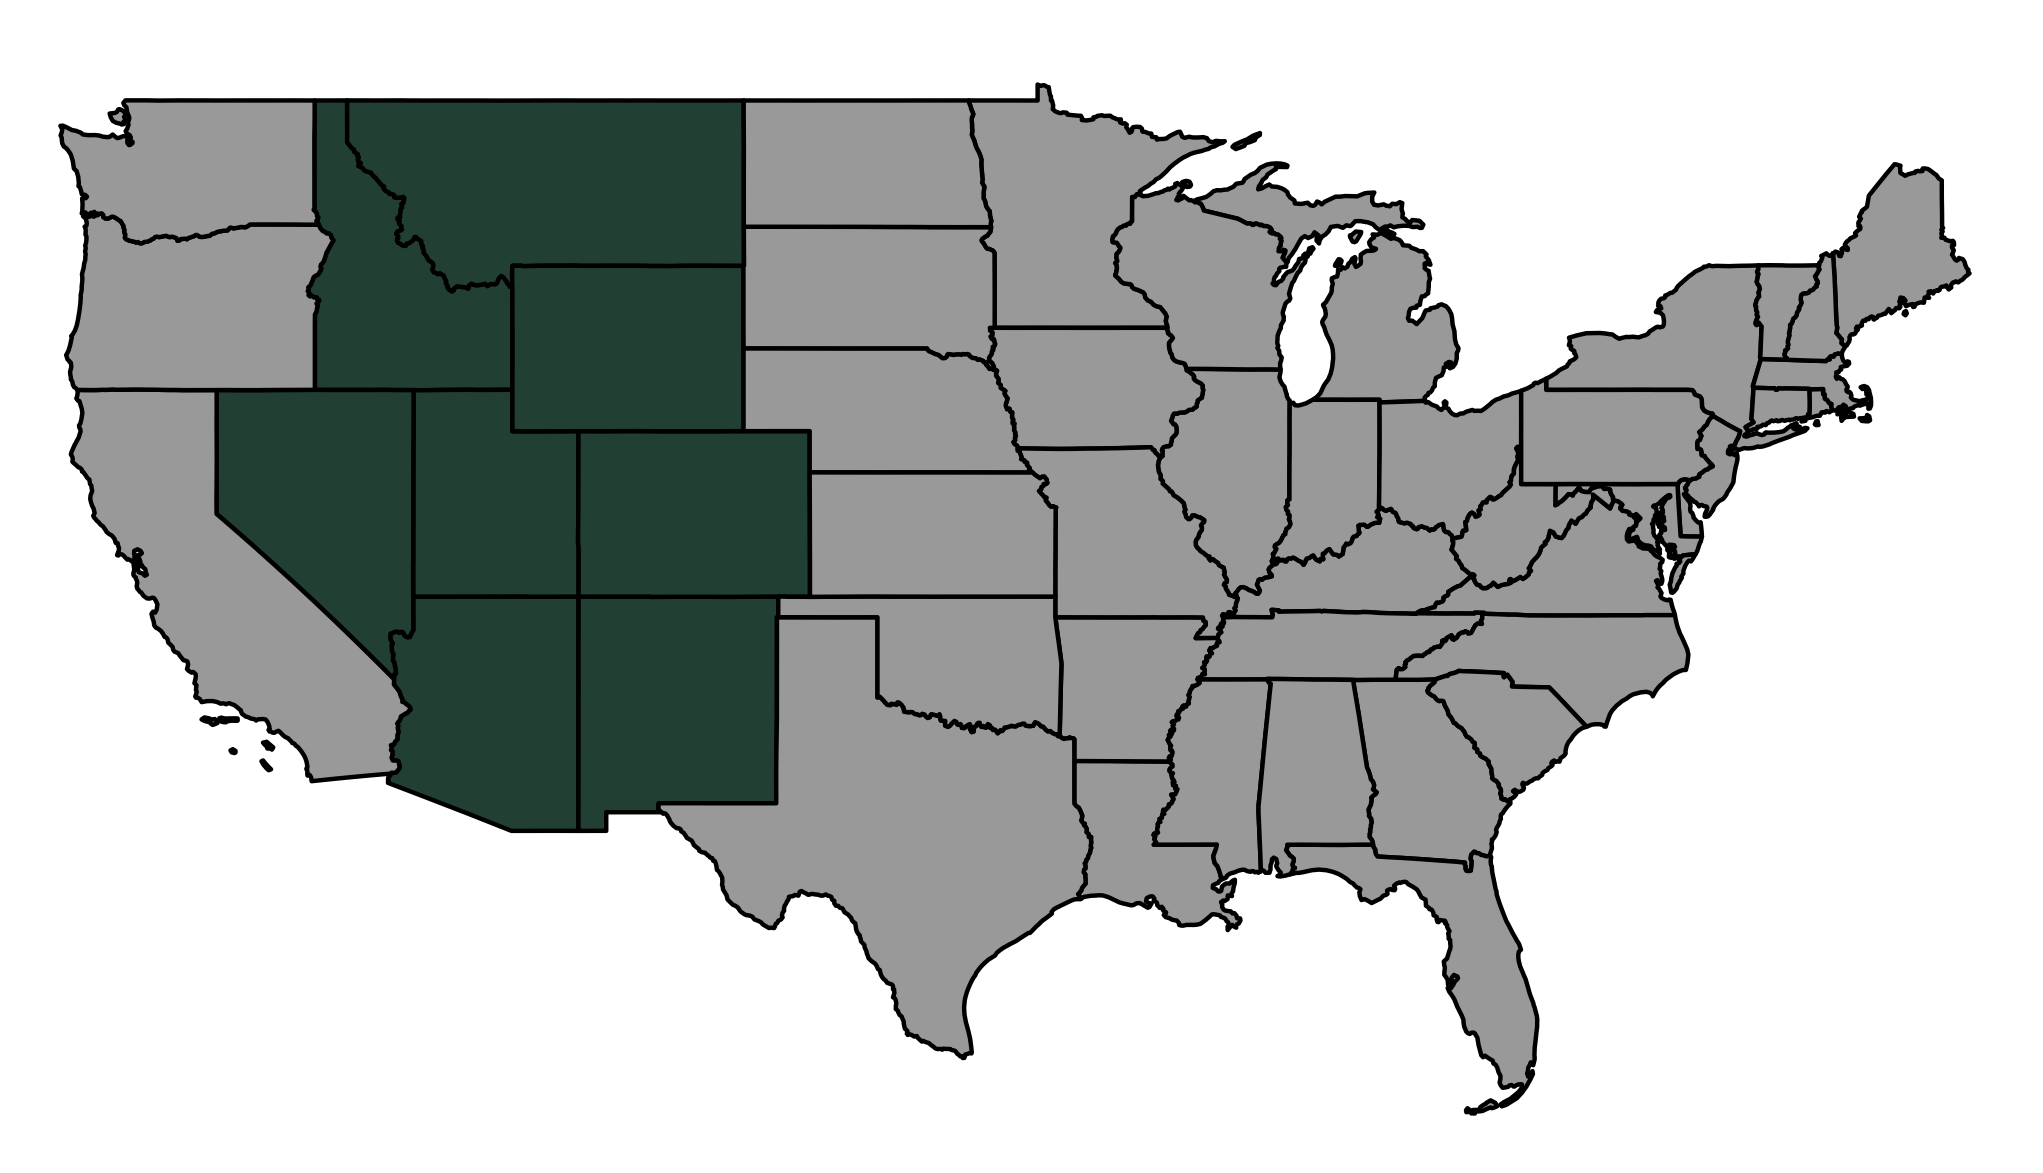
\includegraphics[width=1\linewidth]{figure/interior-west-on-usa} 

}

\caption{The Interior West Region of the United States}\label{fig:unnamed-chunk-3}
\end{figure}
The IW-FIA collects annual inventories of the Interior West, with the goal of covering 10\% of the region each year, so every decade the IW-FIA should have measurement of 100\% of each Interior West state's forests.

The Interior West region itself contains the states which encompass the Rocky Mountains along with some other smaller mountain ranges. The Interior West contains 855,767 square miles of land which has an extremely diverse landscape ranging from the high mountain peaks of the Rockies to flat desert plains in Nevada and other Interior West states. Along with desert and mountains, the Interior West also includes parts of the Great Plains. Throughout this diverse landscape, there is a similarly diverse range of forested areas. The forested areas range from areas that are humid and temperate to areas like the Northern Rocky Mountain Forest which is dry and considered a temperate desert.

\hypertarget{our-data-specifics}{%
\section{Our Data: Specifics}\label{our-data-specifics}}

The data used in this thesis was collected by the Forest Inventory and Analysis Program (FIA) in the span of 10 years from 2007 to 2017. While this data was collected over this 10 year period, the analyses done throughout this thesis are under the assumption that this is a ``snapshot'' of the Interior West at some moment in time. Thus we do not consider any temporal features of this dataset, however the inventory year information is available to us. The data we have is plot-level data for the Interior West region of the United States, where the data for each plot consists of ground data collected by FIA and remotely sensed data.

The dataframe used in this thesis is a joined dataframe derived from two FIA datasets of the Interior West, \texttt{spatial} and \texttt{response}. The \texttt{spatial} dataframe contains 89444 observations and 70 variables, most notably our remotely sensed predictor variable (\texttt{nlcd11}), location information, and ecosubsection. The \texttt{nlcd11} variable was collected by the Multi-Resolution Land Characteristics Consortium (Homer, 2015). This variable measures percent tree canopy cover in a given plot.

The \texttt{response} dataframe contains 86085 observations and 67 variables, most notably four response variables collected by FIA crew members (\texttt{BALIVE\_TPA}, \texttt{CNTLIVE\_TPA}, \texttt{BIOLIVE\_TPA}, and \texttt{VOLNLIVE\_TPA}), location information, and ecosubsection. The response variables noted above measure basal area, tree count, biomass, and volume, respectively. We join these dataframes by their unique plot number, and subset the number of variables significantly to 19 variables which contain plot information, longitude \& lattitude, elevation, predictor variables, response variables, ecosubsection, ecosection, and province. The resulting joined dataframe has 86085 rows as these are the rows which share the same plots between the \texttt{response} and \texttt{spatial} dataframes. We can see the first few rows of the dataframe with relevant columns selected and values rounded to the second decimal place:
\begin{longtable}[t]{rrrrrl}
\caption[Relevant Glimpse of Data]{\label{tab:unnamed-chunk-4}Relevant Glimpse of Data}\\
\toprule
Plot & Latitude & Longitude & nlcd11 & BIOLIVE\_TPA & subsection\\
\midrule
83574 & -109.71 & 32.85 & 21 & 0.00 & 321Af\\
84904 & -109.88 & 32.99 & 0 & 0.00 & 321Af\\
83021 & -109.88 & 32.81 & 0 & 0.00 & 321Aj\\
82635 & -109.89 & 32.65 & 26 & 14.74 & 321Am\\
90381 & -109.83 & 32.62 & 41 & 31.50 & 321Am\\
\addlinespace
81801 & -109.79 & 32.35 & 0 & 0.00 & 321Aj\\
\bottomrule
\end{longtable}
While the data covers the Interior West as a whole, we have very granular information, as each row represents a plot sampled by the FIA. The data also includes variables that subset the Interior West into provinces which contain ecosections, and these ecosections contain ecosubsections. In our data, on average, each ecosection contains approximately 7.06 ecosubsections, and each province contains an average of 4.86 ecosections. So, an average province then contains just over 34 ecosubsections. We can take a look at the Northern Rocky Forest province, colored by ecosection, with lines dividing each ecosubsection to see this structure in action:
\begin{figure}

{\centering 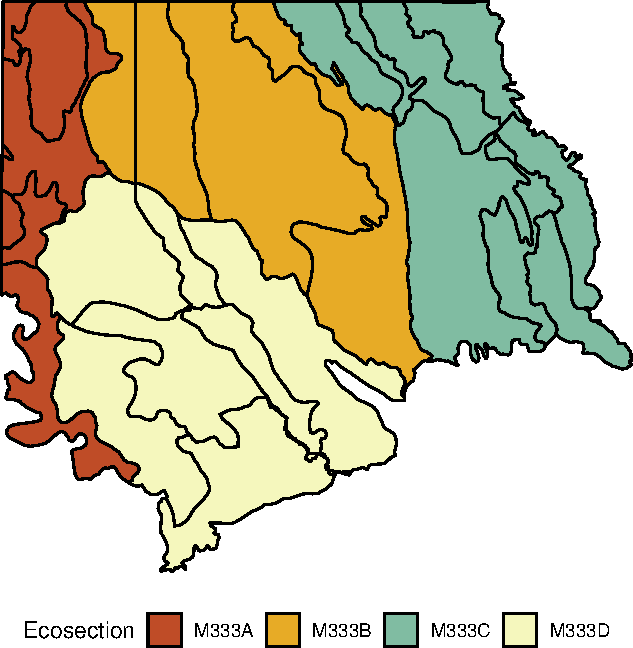
\includegraphics{thesis_files/figure-latex/unnamed-chunk-5-1} 

}

\caption{The Northern Rocky Forest, Colored By Ecosection}\label{fig:unnamed-chunk-5}
\end{figure}
The data we have covers a total of 14 provinces, 68 ecosections, and 480 ecosubsections. The hierarchical struture of the data and nestedness of the ecosubsections within ecosections within provinces lends itself to be able to create hierarchical models which borrow strength from surrounding areas.

While this data contains a multitude of variables, the analyses done in this thesis focus on four key response variables and one explanatory variable. The response variables used are basal area (square-foot), trees per acre, above-ground biomass (lbs), and net volume (ft\^{}3). These variables are coded as \texttt{BALIVE\_TPA}, \texttt{CNTLIVE\_TPA}, \texttt{BIOLIVE\_TPA}, and \texttt{VOLNLIVE\_TPA}, respectively. We can look at the average of these variables across the Interior West region by ecosubsection in the four following maps of the interior west.
\begin{figure}

{\centering 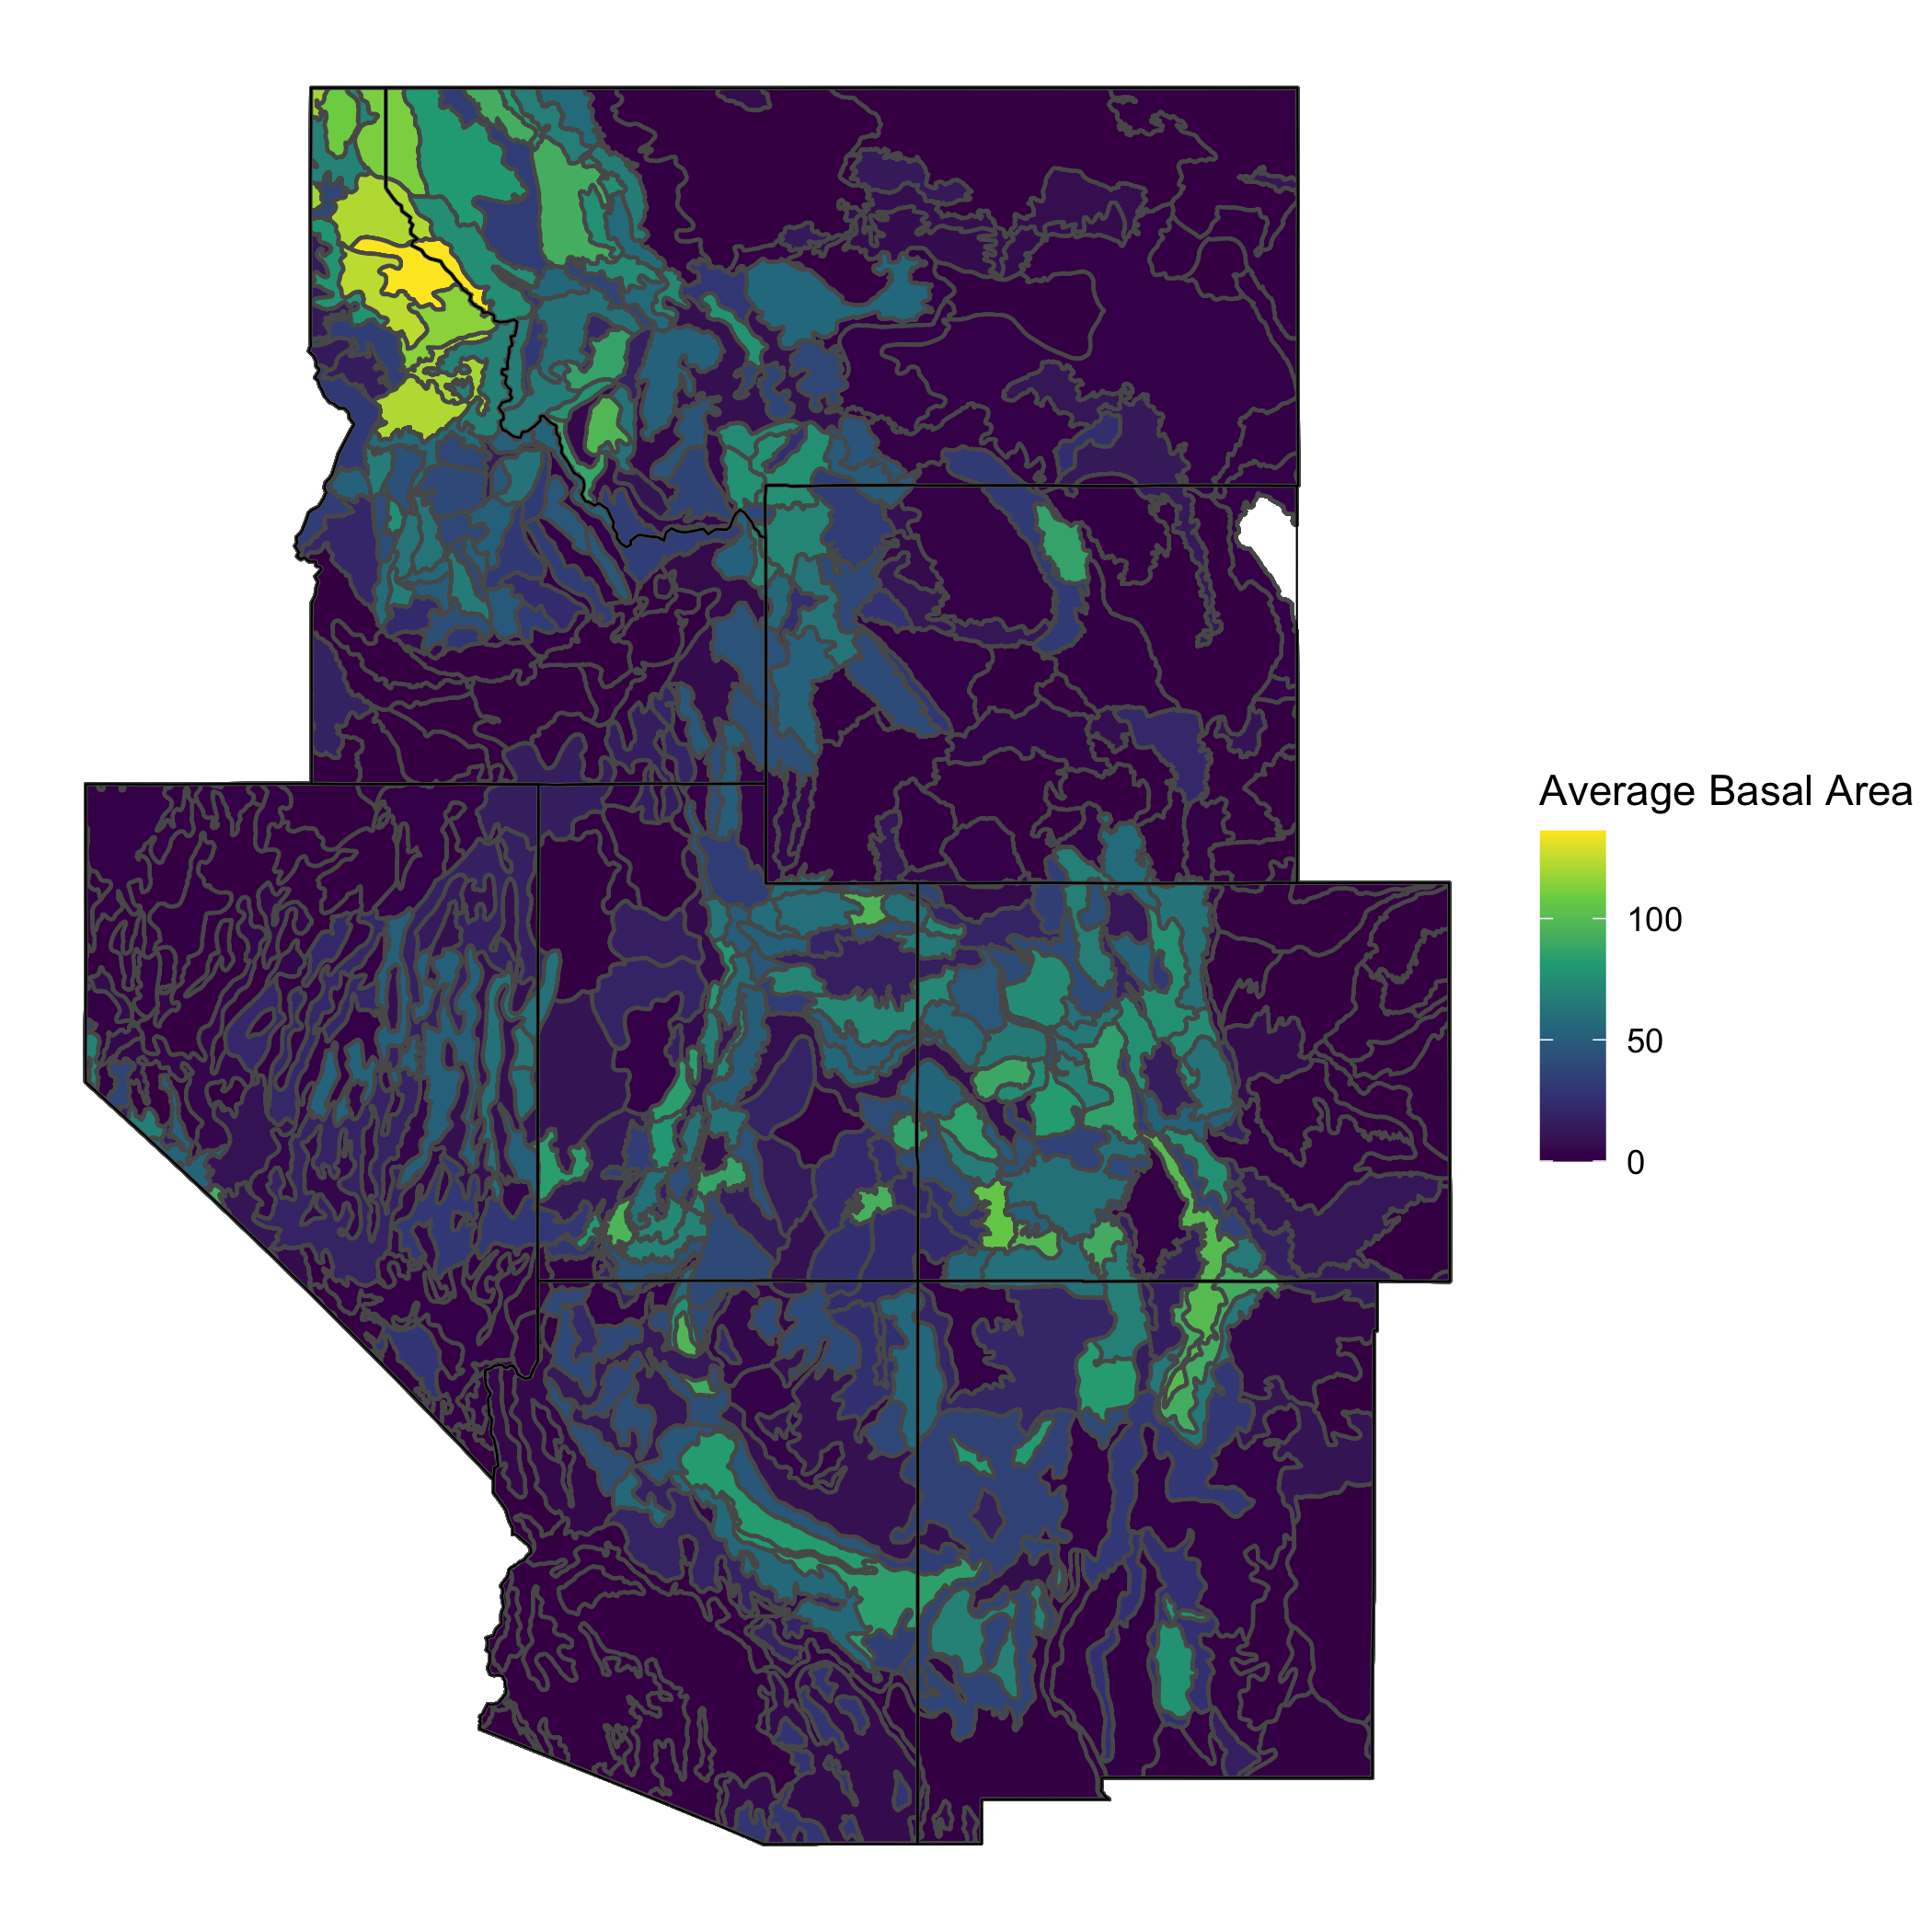
\includegraphics[width=0.65\linewidth]{figure/basal} 

}

\caption{Mean Basal Area in Interior West Ecosubsections}\label{fig:unnamed-chunk-6}
\end{figure}
\begin{figure}

{\centering 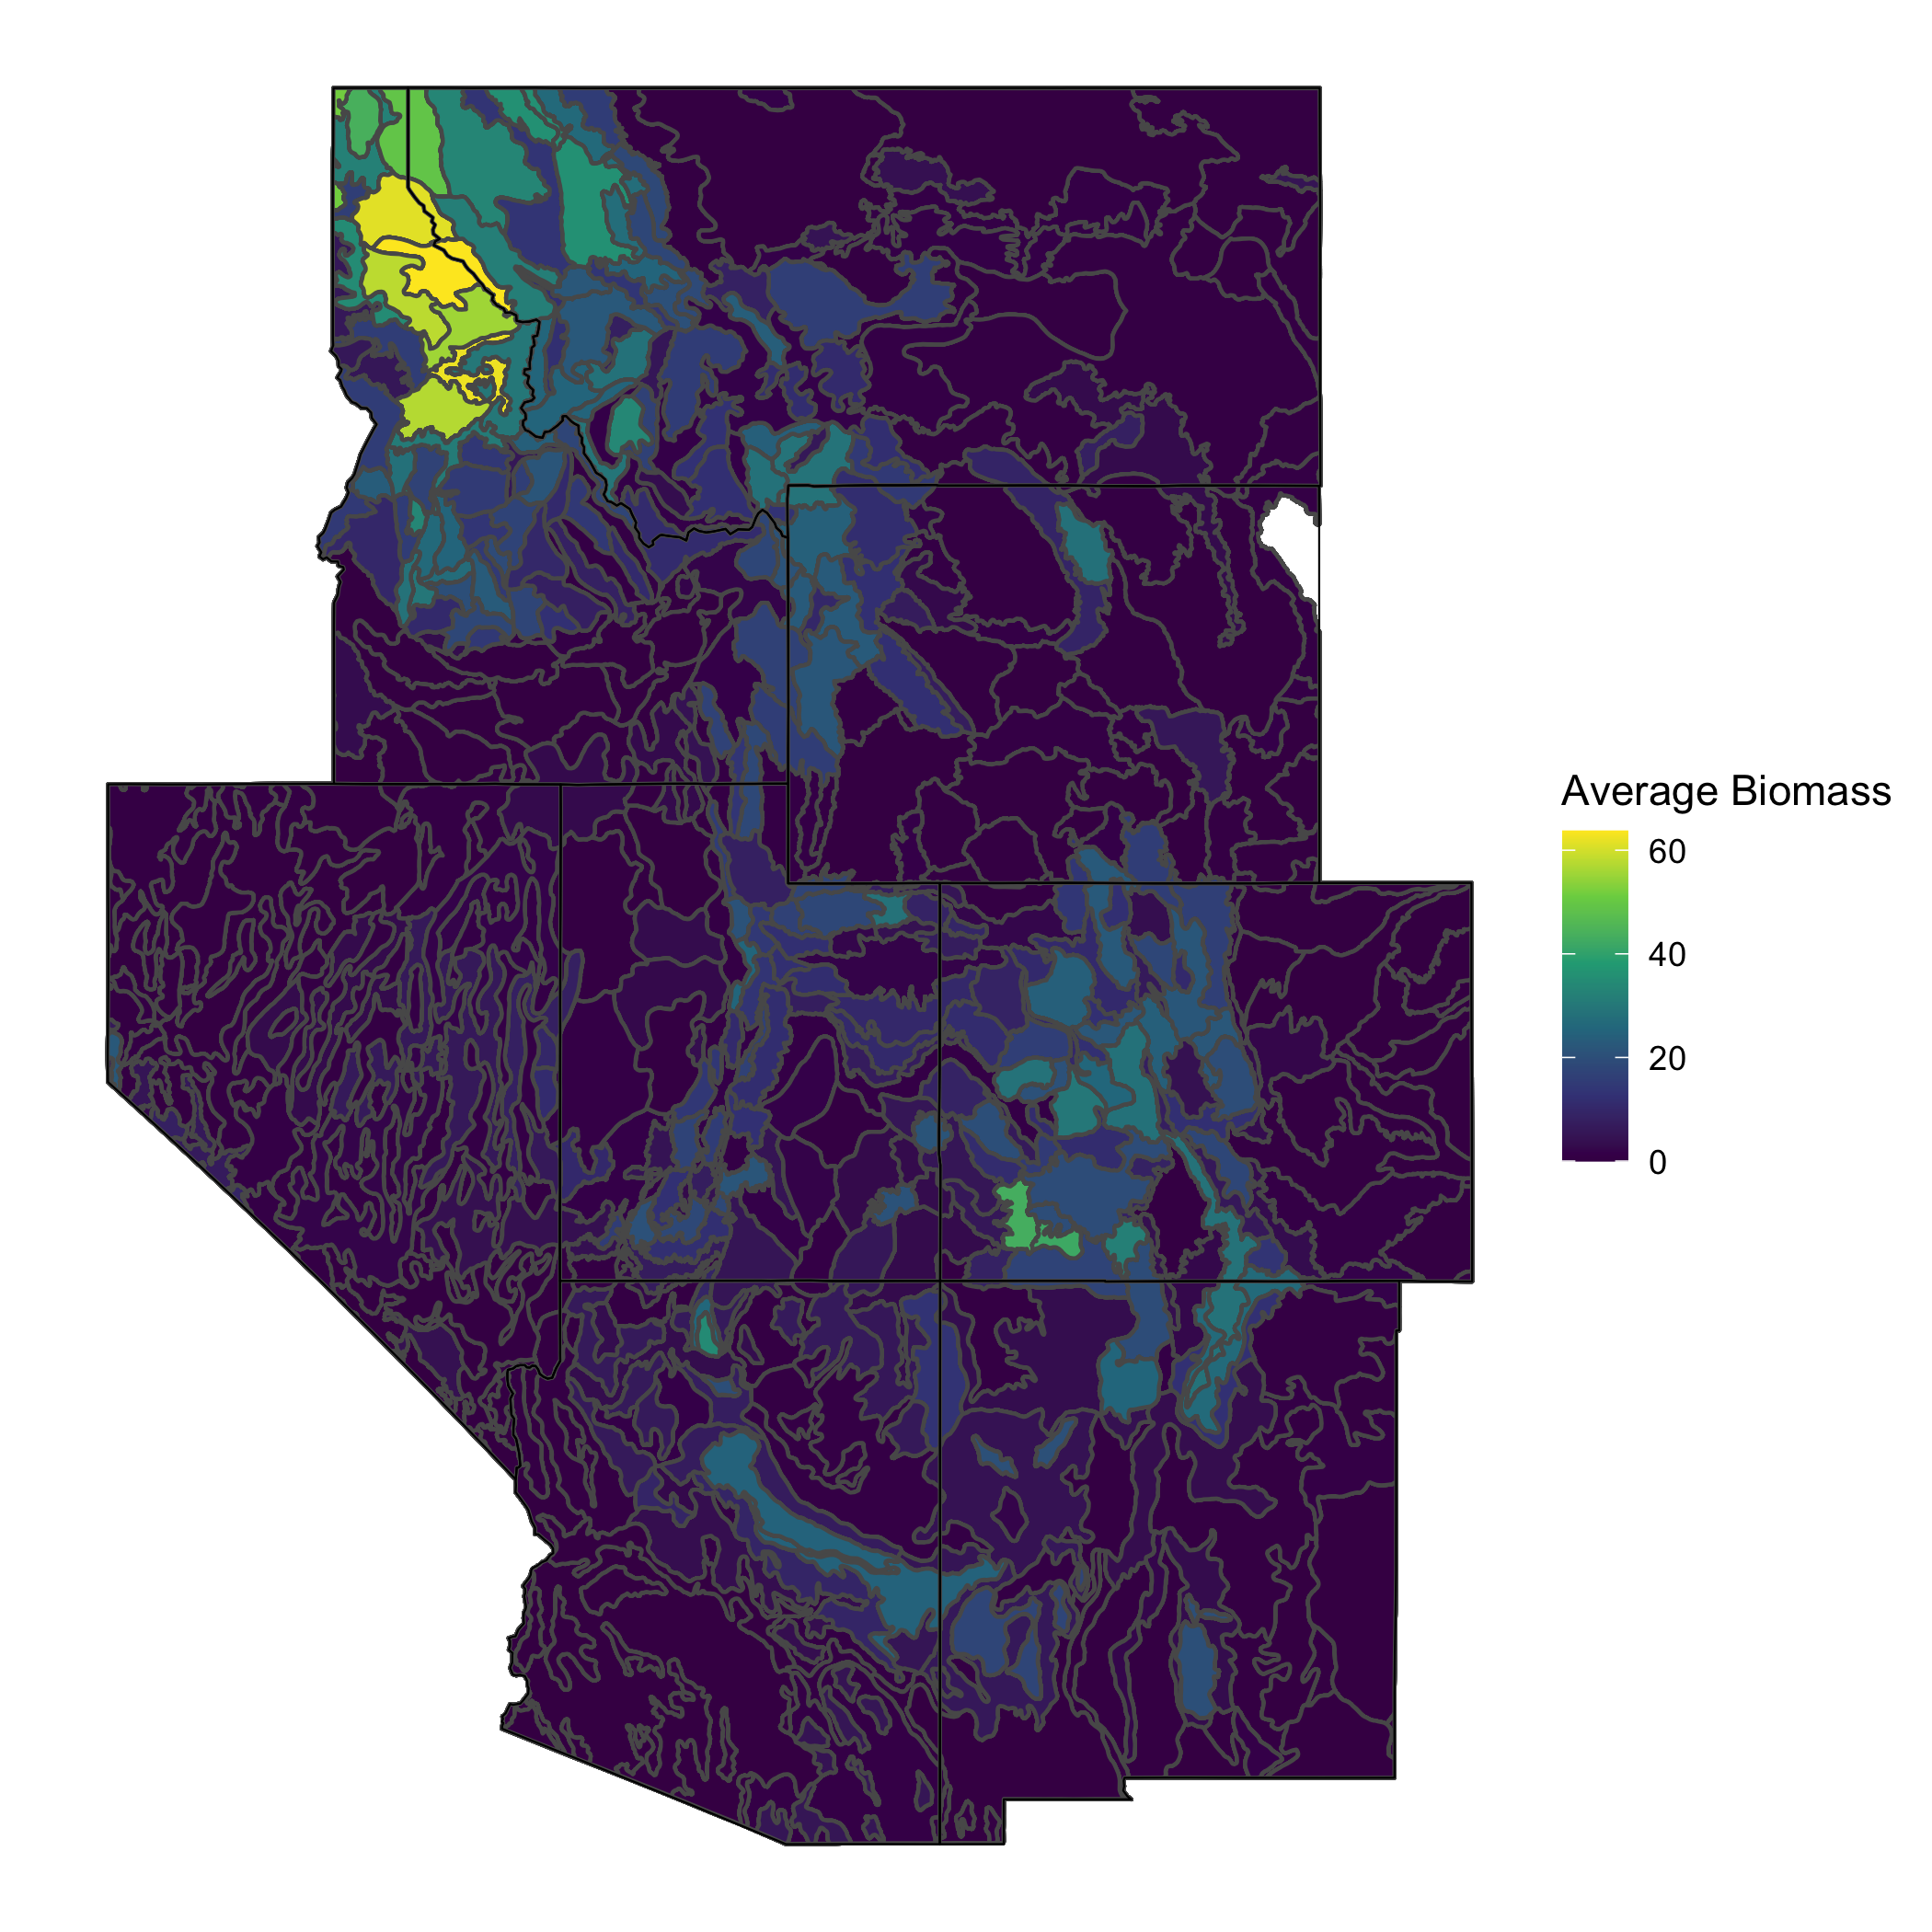
\includegraphics[width=0.65\linewidth]{figure/biomass} 

}

\caption{Mean Biomass in Interior West Ecosubsections}\label{fig:unnamed-chunk-7}
\end{figure}
\begin{figure}

{\centering 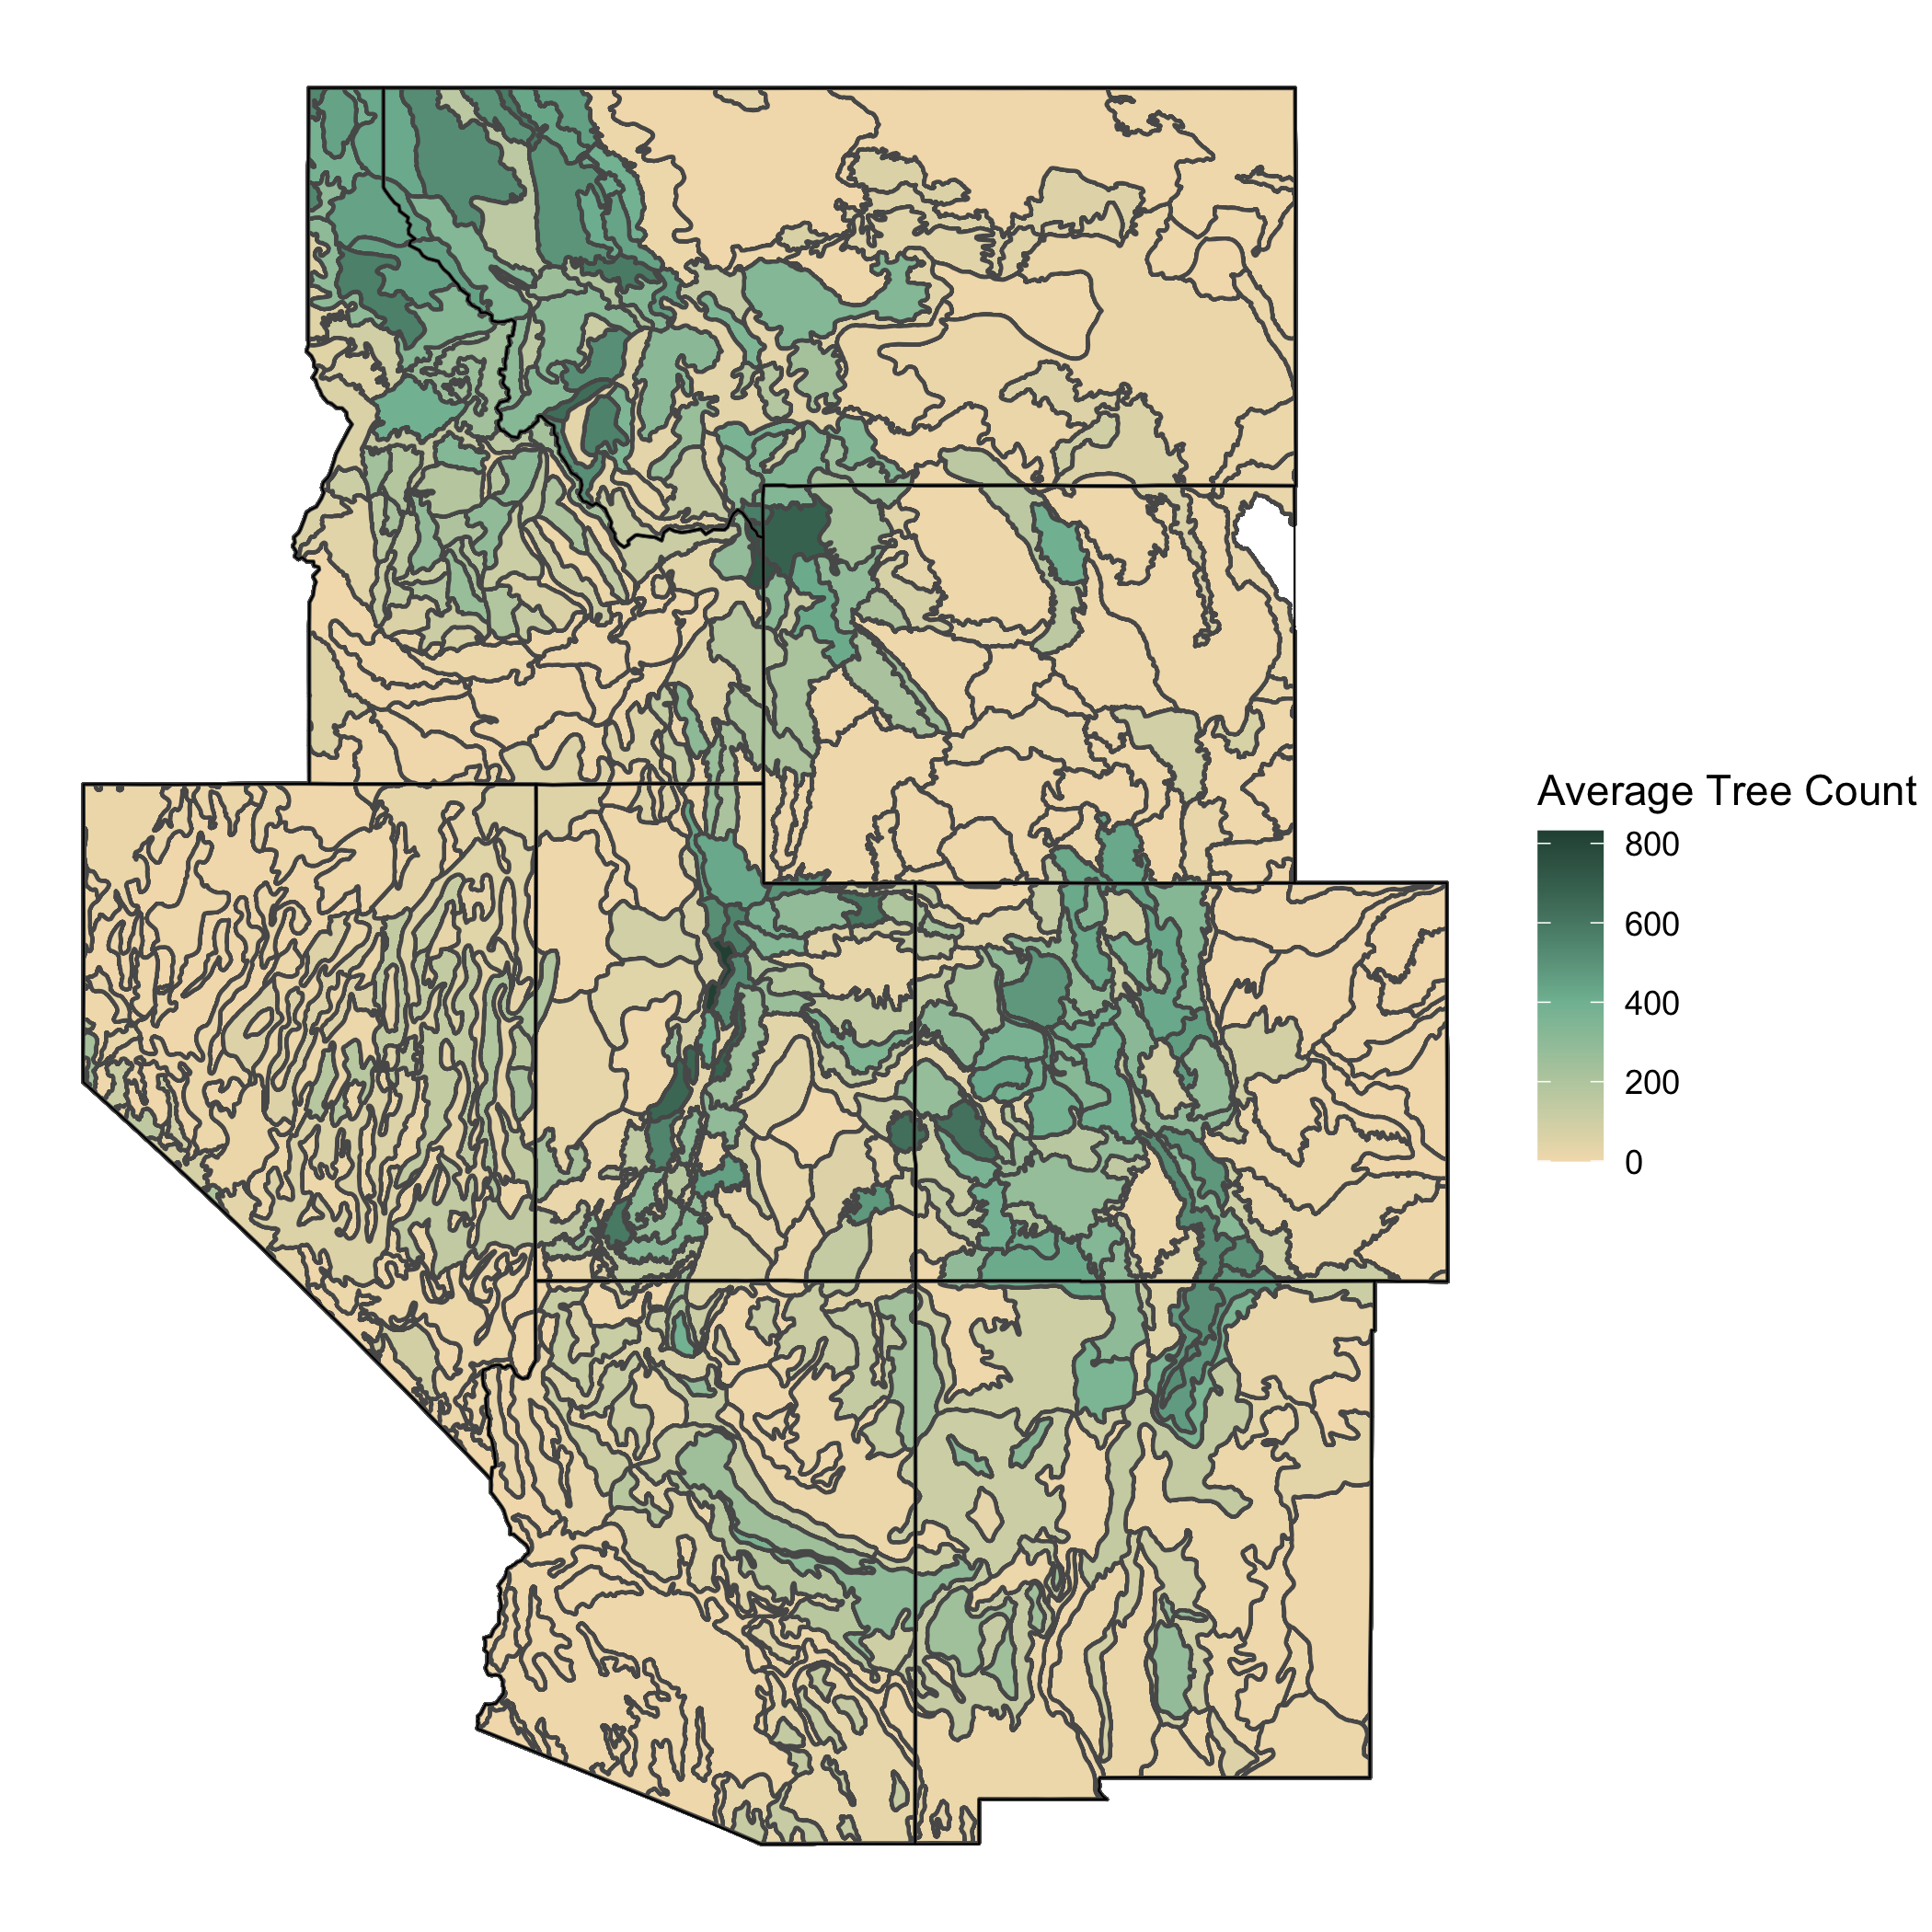
\includegraphics[width=0.65\linewidth]{figure/count} 

}

\caption{Mean Tree Count per acre in Interior West Ecosubsections}\label{fig:unnamed-chunk-8}
\end{figure}
\begin{figure}

{\centering 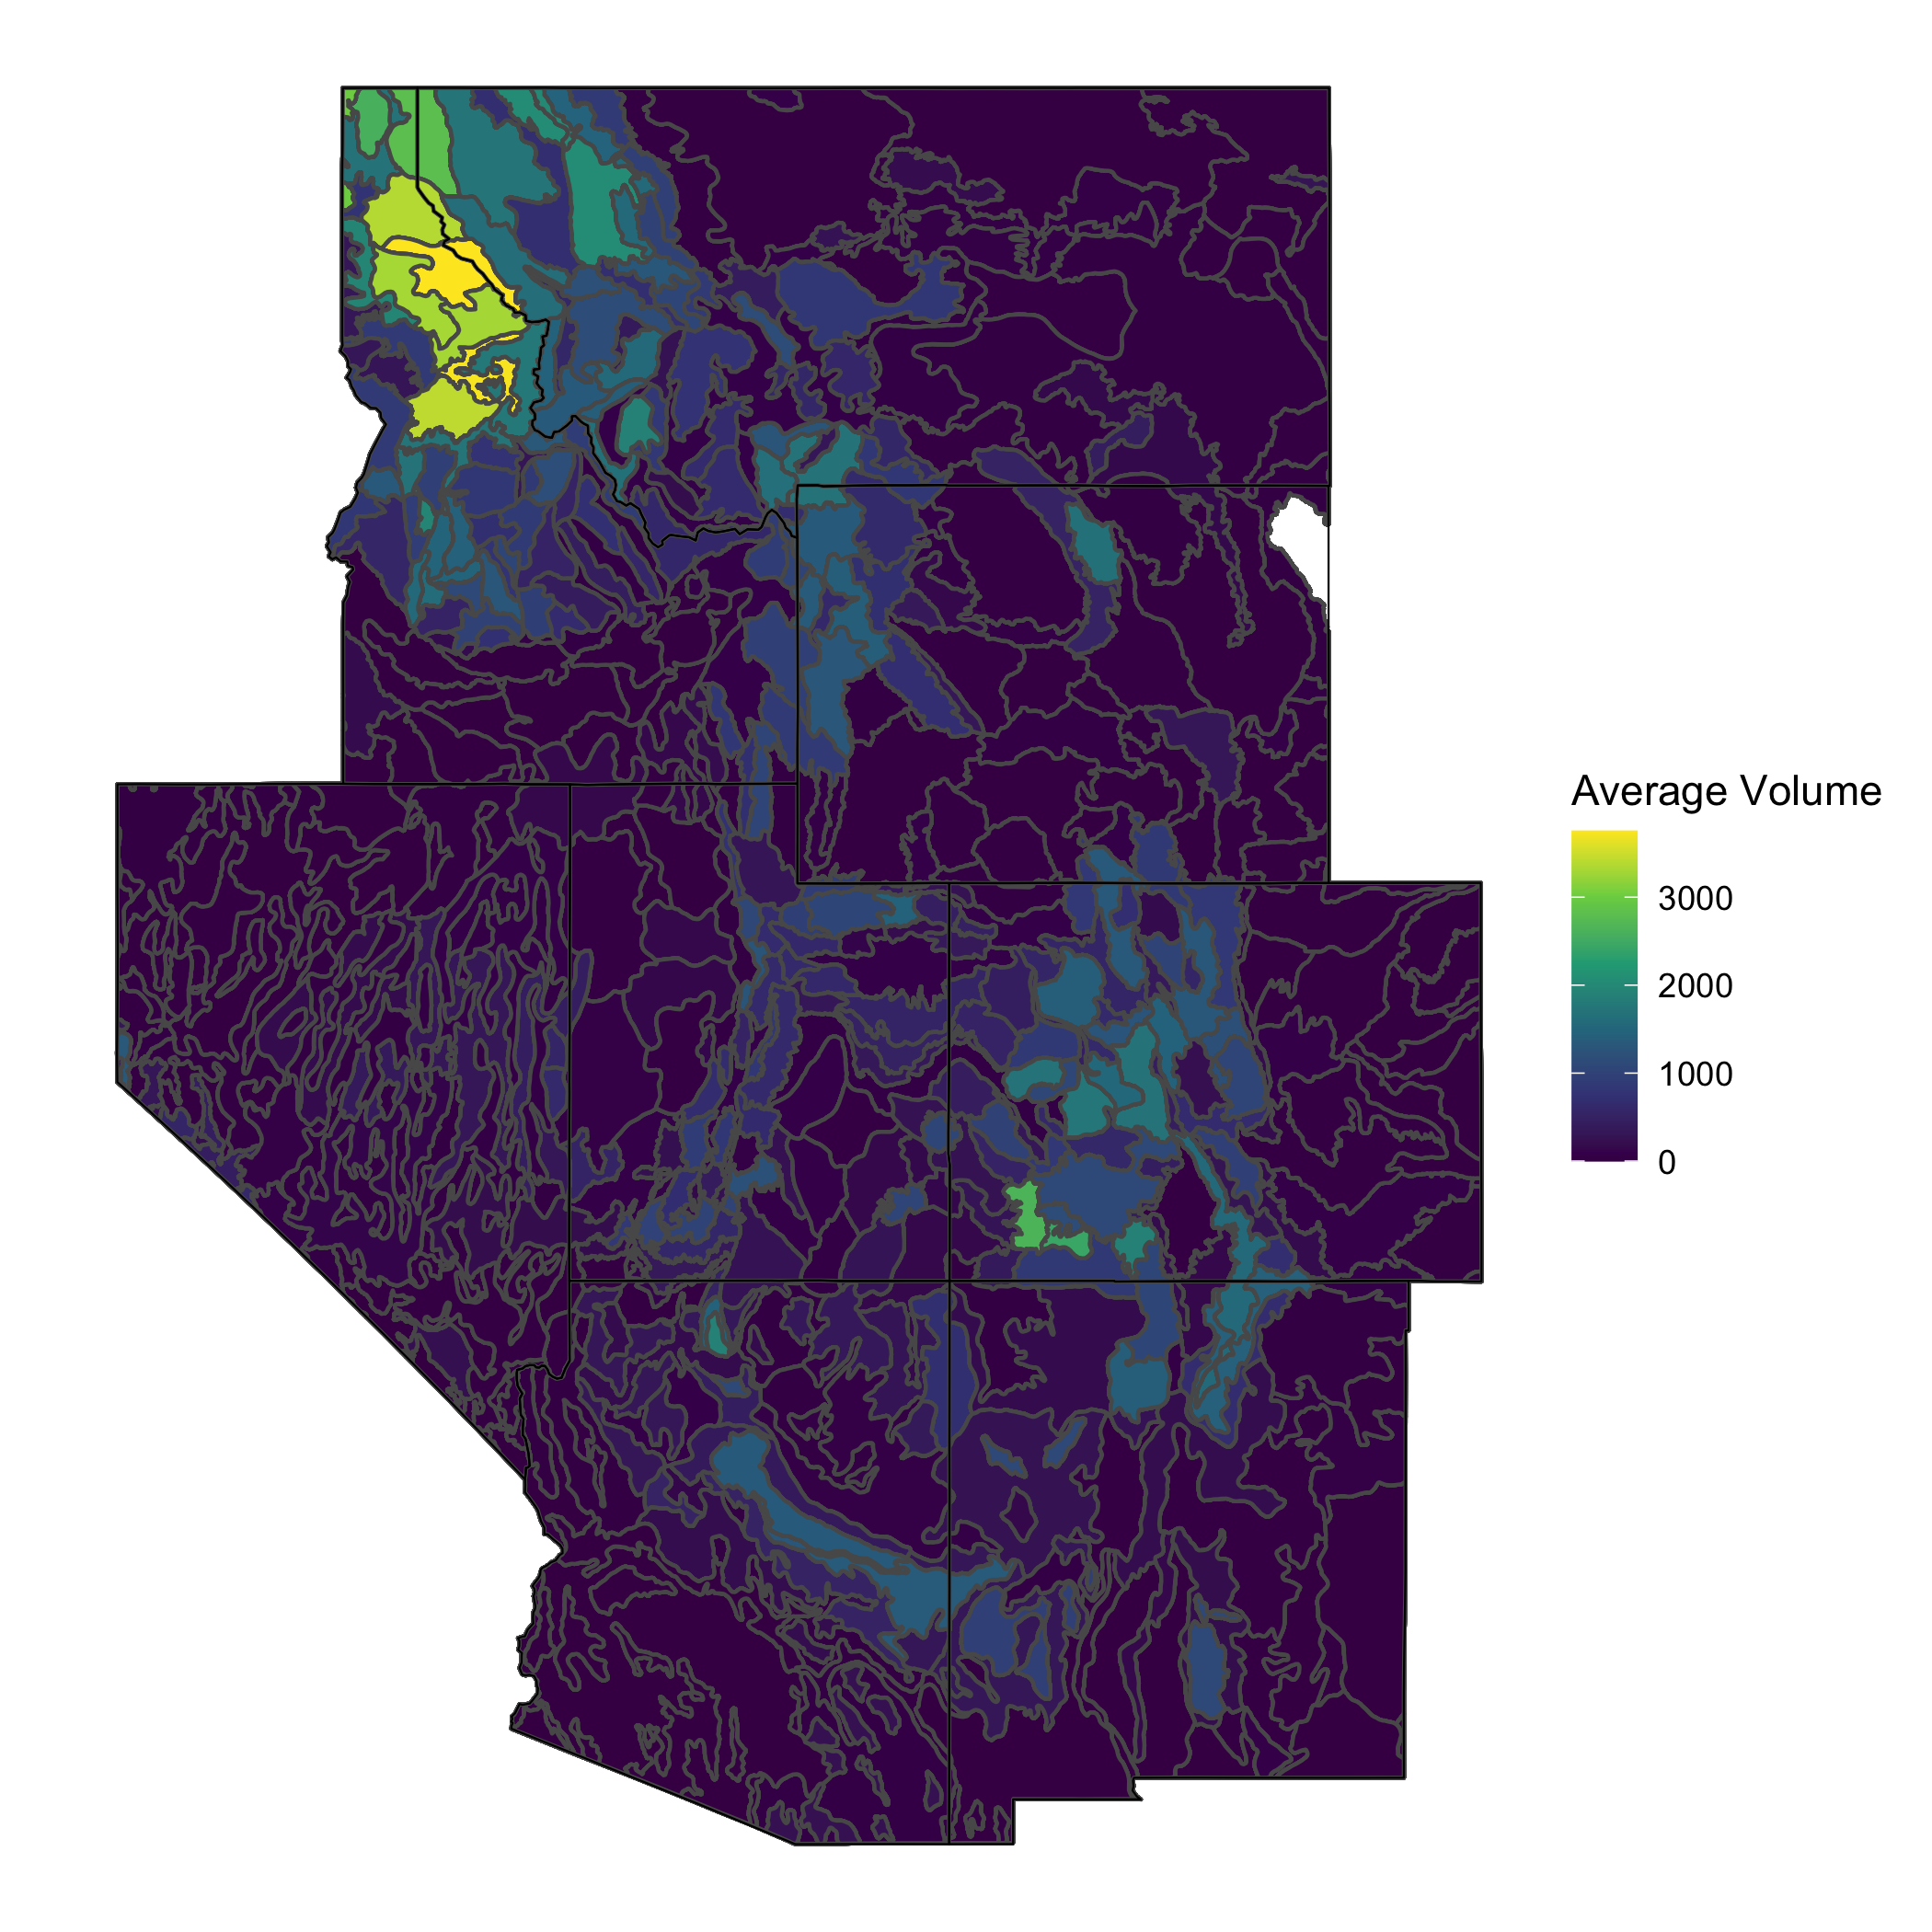
\includegraphics[width=0.65\linewidth]{figure/voln} 

}

\caption{Mean Net Volume in Interior West Ecosubsections}\label{fig:unnamed-chunk-9}
\end{figure}
While we have four variables which we will model as response variables throughout the analyses, we also have one predictor variables which will be of much use to us. In particular, total tree canopy cover (coded as \texttt{nlcd11}.) This variable is remotely sensed, meaning that they were not collected by FIA crew members, but rather with aerial photography and/or satellite imagery. However, we will be using these variables to attempt to predict our response variables in order to understand how good of estimates we can make with this remote data that does not require as much effort to collect.

To get a sense of a few of our predictor variable, we will look at its distributions in the Northern Rocky Forest subset of our data compared to its distribution across the entire Interior West:
\begin{figure}

{\centering 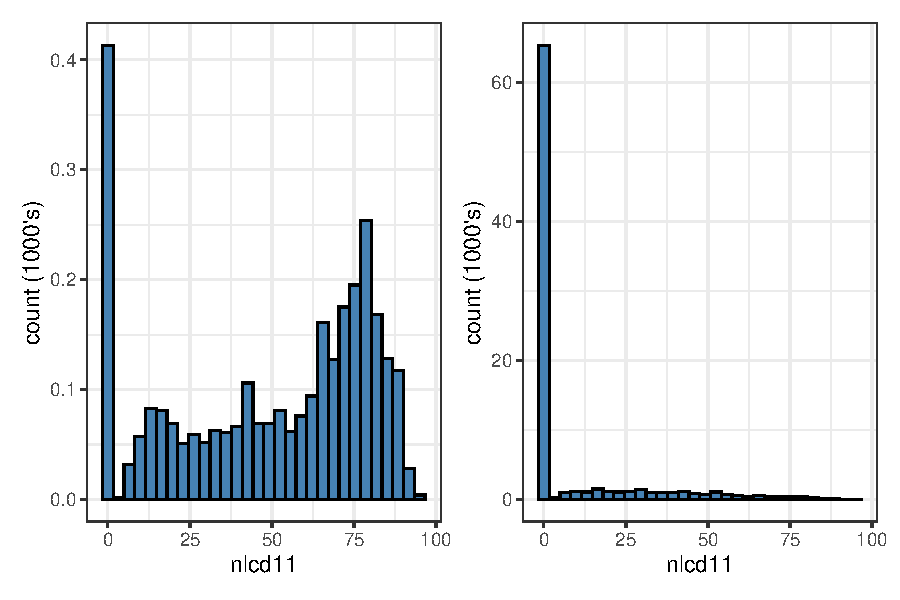
\includegraphics[width=432px]{thesis_files/figure-latex/unnamed-chunk-10-1} 

}

\caption{Distribution of Total Canopy Cover in the M333 Province (Top) and the Entire Interior West (Bottom)}\label{fig:unnamed-chunk-10}
\end{figure}
Notably, the Northern Rocky Forest Province (M333) is much more forested than the Interior West, so we see much different distributions of total canopy cover in this subset of the data. Apart from making these histograms, we can also summarize the entire, unit-level data and see some summary statistics of our five key variables:
\begin{longtable}[t]{lrrrrrr}
\caption[Summary Statistics of Relevant Variables]{\label{tab:unnamed-chunk-11}Summary Statistics of Relevant Variables}\\
\toprule
Variable & Mean & SD & Median & 75th Percentile & Min & Max\\
\midrule
nlcd11 & 8.73 & 18.57 & 0 & 0.00 & 0 & 95.00\\
BIOLIVE\_TPA & 6.23 & 16.84 & 0 & 1.98 & 0 & 244.35\\
BALIVE\_TPA & 22.75 & 48.06 & 0 & 14.75 & 0 & 469.39\\
CNTLIVE\_TPA & 98.60 & 283.09 & 0 & 30.09 & 0 & 6677.93\\
VOLNLIVE\_TPA & 342.32 & 972.78 & 0 & 74.69 & 0 & 16435.55\\
\bottomrule
\end{longtable}
From this table, we can see how heavily skewed these key variables are, with all the variables having median of zero. This does not stop us from doing meaningful analyses though, as the sample size of this dataset is so large (\(n = 86085\)) and thus we have plenty of data to create models with.

\hypertarget{data-structure-hierarchy}{%
\section{Data Structure \& Hierarchy}\label{data-structure-hierarchy}}

As hinted at throughout earlier parts of the chapter, the data used in this thesis has a hierarchical structure, where ecosubsections are nested within ecosections which are in turn nested within provinces. Every plot has each level of granularity of location data recorded and this is what allows us to choose how far to borrow strength from other plots. We can see this structure of nested data by looking at an example up close of Idaho's ecosubsections colored by their province, and then their ecosection:
\begin{figure}

{\centering 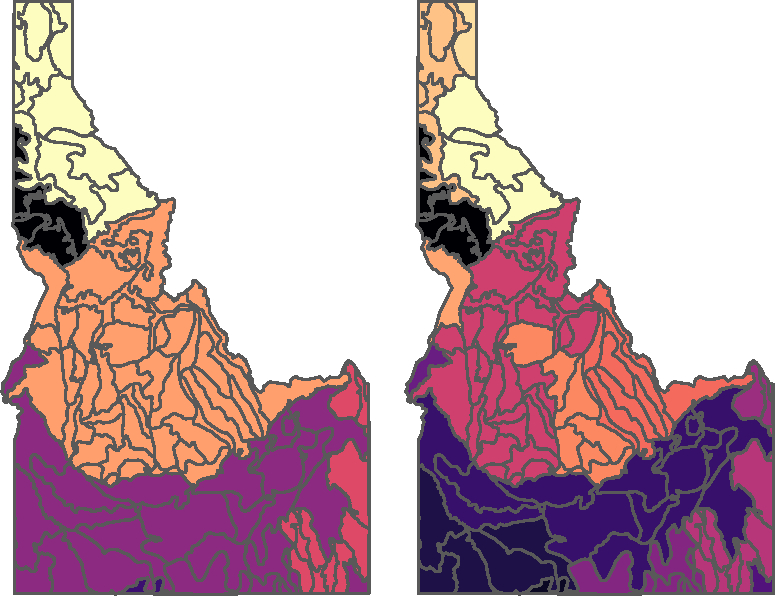
\includegraphics{thesis_files/figure-latex/unnamed-chunk-12-1} 

}

\caption{Idaho Colored by Province (Left) and Ecosection (Right)}\label{fig:unnamed-chunk-12}
\end{figure}
The largest motivation for hierarchical modeling in this particular application is that observations are more similar within the hierarchies which we split them into. To understand if this is true, we can do a preliminary analysis on the data by performing three-way ANOVAs for each key variable with predictors \texttt{province}, \texttt{section}, and \texttt{subsection}. For succintness, we can look at the ANOVA results for one of the repsonse variables, \texttt{BIOLIVE\_TPA}, but the other variables tell a very similar story in terms of homogeneity. By just looking at the MSE of the ANOVA results, we can see that we should expect more homogeneity within ecosubsections:
\begin{longtable}[]{@{}cccccc@{}}
\caption{Analysis of Variance Model (Biomass Response)}\tabularnewline
\toprule
\begin{minipage}[b]{0.15\columnwidth}\centering
term\strut
\end{minipage} & \begin{minipage}[b]{0.09\columnwidth}\centering
df\strut
\end{minipage} & \begin{minipage}[b]{0.13\columnwidth}\centering
sumsq\strut
\end{minipage} & \begin{minipage}[b]{0.10\columnwidth}\centering
meansq\strut
\end{minipage} & \begin{minipage}[b]{0.14\columnwidth}\centering
statistic\strut
\end{minipage} & \begin{minipage}[b]{0.14\columnwidth}\centering
p.value\strut
\end{minipage}\tabularnewline
\midrule
\endfirsthead
\toprule
\begin{minipage}[b]{0.15\columnwidth}\centering
term\strut
\end{minipage} & \begin{minipage}[b]{0.09\columnwidth}\centering
df\strut
\end{minipage} & \begin{minipage}[b]{0.13\columnwidth}\centering
sumsq\strut
\end{minipage} & \begin{minipage}[b]{0.10\columnwidth}\centering
meansq\strut
\end{minipage} & \begin{minipage}[b]{0.14\columnwidth}\centering
statistic\strut
\end{minipage} & \begin{minipage}[b]{0.14\columnwidth}\centering
p.value\strut
\end{minipage}\tabularnewline
\midrule
\endhead
\begin{minipage}[t]{0.15\columnwidth}\centering
province\strut
\end{minipage} & \begin{minipage}[t]{0.09\columnwidth}\centering
13\strut
\end{minipage} & \begin{minipage}[t]{0.13\columnwidth}\centering
6512457\strut
\end{minipage} & \begin{minipage}[t]{0.10\columnwidth}\centering
500958\strut
\end{minipage} & \begin{minipage}[t]{0.14\columnwidth}\centering
2921\strut
\end{minipage} & \begin{minipage}[t]{0.14\columnwidth}\centering
0\strut
\end{minipage}\tabularnewline
\begin{minipage}[t]{0.15\columnwidth}\centering
section\strut
\end{minipage} & \begin{minipage}[t]{0.09\columnwidth}\centering
54\strut
\end{minipage} & \begin{minipage}[t]{0.13\columnwidth}\centering
967169\strut
\end{minipage} & \begin{minipage}[t]{0.10\columnwidth}\centering
17911\strut
\end{minipage} & \begin{minipage}[t]{0.14\columnwidth}\centering
104.4\strut
\end{minipage} & \begin{minipage}[t]{0.14\columnwidth}\centering
0\strut
\end{minipage}\tabularnewline
\begin{minipage}[t]{0.15\columnwidth}\centering
subsection\strut
\end{minipage} & \begin{minipage}[t]{0.09\columnwidth}\centering
412\strut
\end{minipage} & \begin{minipage}[t]{0.13\columnwidth}\centering
2247965\strut
\end{minipage} & \begin{minipage}[t]{0.10\columnwidth}\centering
5456\strut
\end{minipage} & \begin{minipage}[t]{0.14\columnwidth}\centering
31.82\strut
\end{minipage} & \begin{minipage}[t]{0.14\columnwidth}\centering
0\strut
\end{minipage}\tabularnewline
\begin{minipage}[t]{0.15\columnwidth}\centering
Residuals\strut
\end{minipage} & \begin{minipage}[t]{0.09\columnwidth}\centering
85605\strut
\end{minipage} & \begin{minipage}[t]{0.13\columnwidth}\centering
14679154\strut
\end{minipage} & \begin{minipage}[t]{0.10\columnwidth}\centering
171.5\strut
\end{minipage} & \begin{minipage}[t]{0.14\columnwidth}\centering
NA\strut
\end{minipage} & \begin{minipage}[t]{0.14\columnwidth}\centering
NA\strut
\end{minipage}\tabularnewline
\bottomrule
\end{longtable}
These results allow us to conclude that it is reasonable to believe that observations within a given province are more homogeneous than observations throughout the Interior West. Thus, if we want ecosubsection level estimates of variables, it makes sense to borrow information from other ecosubsections within the same province as each other. This data structure and homogeneity within provinces is what drives the analyses done henceforth in this thesis.

\hypertarget{methods}{%
\chapter{Methods}\label{methods}}

Gives an overview of the current main approaches to the problem.
Points out flaws in existing approaches and addresses how the current work mitigates these problems

These are models which are often fit by maximum likelihood estimation and other methods of maximizing the likelihood function such are restricted maximum likelihood estimation. The likelihood can be written as
\[
P(X ~\vert ~ \theta)
\]
where \(X\) is the data and \(\theta\) is the parameter of interest. Note that the likelihood function allows the value of \(X\) to vary while the parameter, \(\theta\), is considered a fixed value. The other school of statistical thought, Bayesian statistics, considers the parameter of interest as varying while the considering the data as fixed. We call this the posterior distribution of \(\theta\), and Bayes' theorem gives us the following relation
\[
P(\theta ~\vert ~ X) = \frac{P(X ~\vert ~ \theta) P(\theta)}{P(X)}
\]

\hypertarget{results}{%
\chapter{Results}\label{results}}

\hypertarget{modeling-overview}{%
\section{Modeling Overview}\label{modeling-overview}}

We explore both unit- and area-level models in this thesis, where unit-level models fit the model to the plot (unit) level data, and the area-level models fit to data which has been aggregated to the ecosubsection (area) level. These models types each have their own costs and benefits, and while we lose some data structure with the area-level estimates we gain a large amount of precision. We can see this when looking at the correlation between the predictor \texttt{nlcd11} and one of our response variables, \texttt{BIOLIVE\_TPA}, at both the unit- and area-levels with ordinary least squares regression lines fit to the data:
\begin{figure}

{\centering 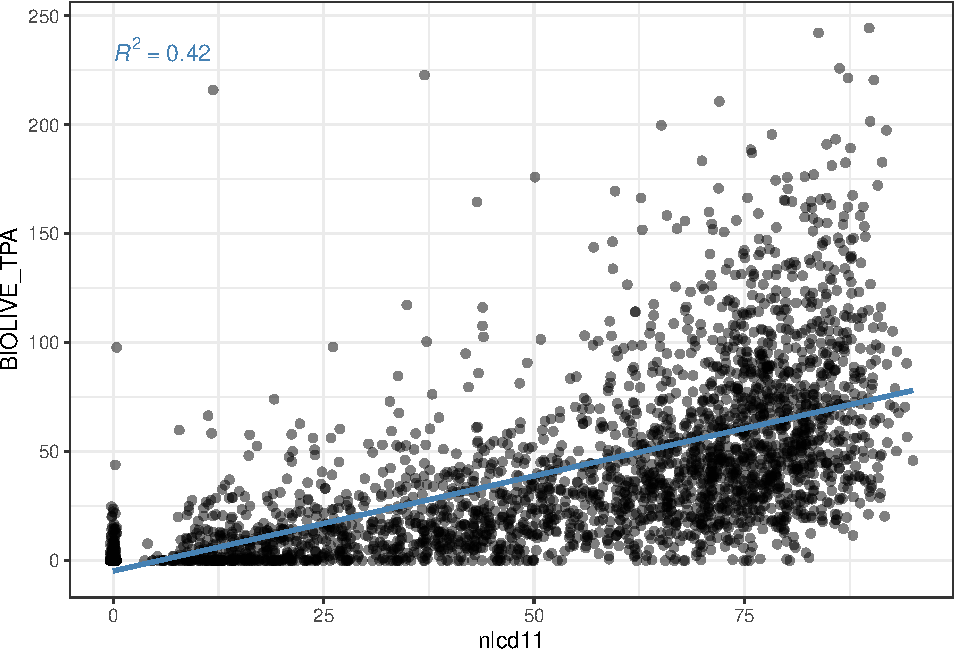
\includegraphics[width=0.9\linewidth]{thesis_files/figure-latex/unnamed-chunk-15-1} 

}

\caption{Unit-level correlation}\label{fig:unnamed-chunk-15}
\end{figure}
\begin{figure}

{\centering 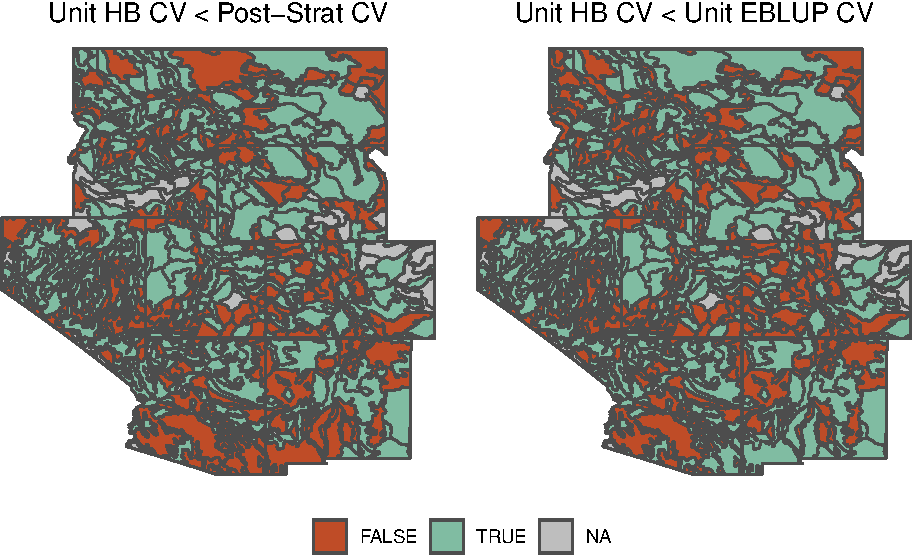
\includegraphics[width=0.9\linewidth]{thesis_files/figure-latex/unnamed-chunk-16-1} 

}

\caption{Area-level correlation}\label{fig:unnamed-chunk-16}
\end{figure}
Notably, the \(R^2\) value for the area-level simple linear regression is much higher than the \(R^2\) value at the unit-level. This is of course compromised by the number of data points (\(n_{area} = 20, ~ n_{unit} = 3003\)). Also, fitting a polynomial regression curve to the unit level data hardly improves the fit (\(R^2 = 0.44\)).

We, however, are not fitting simple linear regressions. In this chapter, we explore the benefits of Bayesian hierarchical models which use varying-slopes to lower the variance in our estimates at the cost of a small amount of bias.

\hypertarget{unit-level-models}{%
\section{Unit-level Models}\label{unit-level-models}}

At the unit-level, the small area estimates for each ecosubsection are made by post-aggregation of the plot level output of our model. We fit these models using varying slopes model, which can be written as:
\begin{align*}
Y_i &\sim N(\alpha_j + \vec\beta\vec X_i,~ \sigma^2) \\
\alpha_j &\sim N(\mu_\alpha,~ \sigma^2_\alpha) \\
\mu_\alpha &\sim N(a,~b)
\end{align*}
Here, we have \(Y_i\), our response variable (\texttt{BIOLIVE\_TPA}), which is modeled to have a Gaussian posterior distribution with mean \(\alpha_j + \vec\beta\vec X_i\) which can change intercept based on the level that a given observation is in. Note that we are predicting \(Y\) at the unit-level, so we compute \(Y_i\) for every plot in the Northern Rocky Forest, and we allow \(\alpha_j\), the intercept, to vary over each of the 20 ecosubsections within the Northern Rocky Forest. Then, we must aggregate our result by taking the mean of our \(Y_i\)'s in each small area. After fitting this model and preforming the aggregation, we can look at the estimates of the mean biomass predicted by the model compared to the direct estimator:
\begin{figure}

{\centering 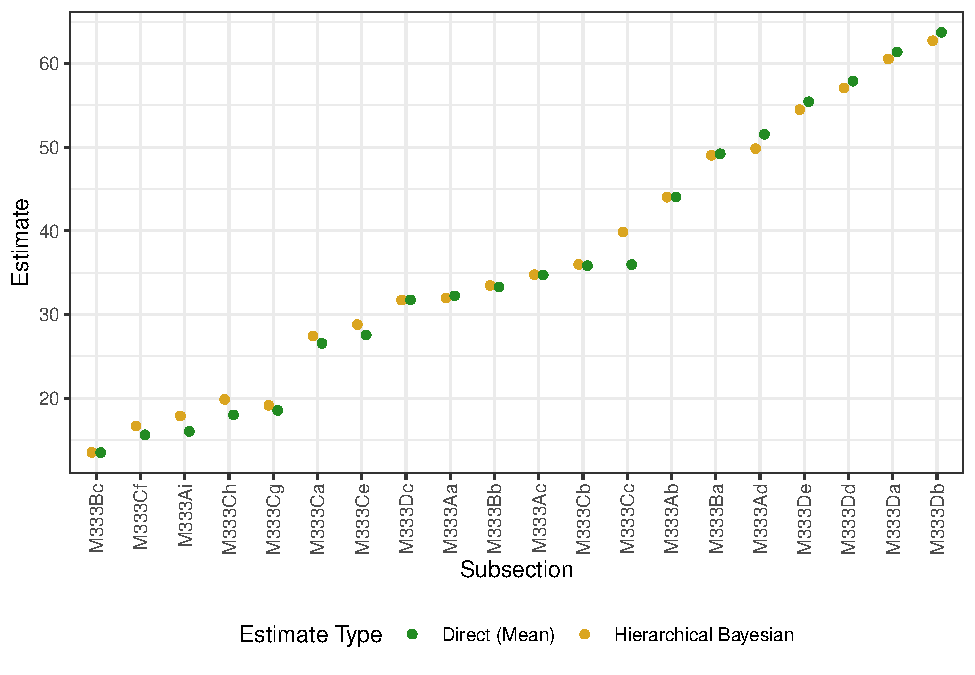
\includegraphics[width=0.9\linewidth]{thesis_files/figure-latex/unnamed-chunk-17-1} 

}

\caption{Direct and model-based estimates for the unit-level model}\label{fig:unnamed-chunk-17}
\end{figure}
These estimates make sense in the context of hierarhical Bayesian modeling because we can see the shrinkage of the estimates towards the overall mean. We also see more shrinkage in ecosubsections which have less plots, particularly M333Cc (\(n_j = 28\)), M333Ai (\(n_j = 38\)), and M333Ad (\(n_j = 26\)). This is again consistent with our intuition as small areas with less data should rely more heavily on the overall mean biomass level of the Northern Rocky Forest.

We can also begin to look at the increase in precision which is gained from this unit-level hierarchial Bayesian model by examining the coefficient of variation for the model and the direct estimator in each ecosubsection. For the direct estimator, the coefficient of variation of a certain ecosubsection \(j\) is defined as
\begin{align}
CV_{\text{direct}} = \frac{\sqrt{\text{var}(Y_{i,j})}}{\text{mean}(Y_{i,j})}
\end{align}
where \(Y_{i,j}\) considers all \(i = 1,\dots,n_j\) units in the \(j\)th ecosubsection. Similarly, for the model-based estimator we define the coefficient of variation as
\begin{align}
CV_{\text{model}} = \frac{\sqrt{\frac{1}{n}\sum_{i=1}^{n_j} (Y_{i,j} - \hat{Y}_{i,j})^2}}{\text{mean}(Y_{i,j})}
\end{align}
Note that the numerator is now the root mean squared error of the \(j\)th ecosubsection. This is equvalent to taking the square root of the variance as we did in the direct estimator's coefficent of variation, given that our model perfectly meets our modeling assumptions. Knowing that this will never perfectly be the case, we take the root mean squared error to get a more realistic estimate. Now, we can visualize this statisitc for each ecosubsection:
\begin{figure}

{\centering 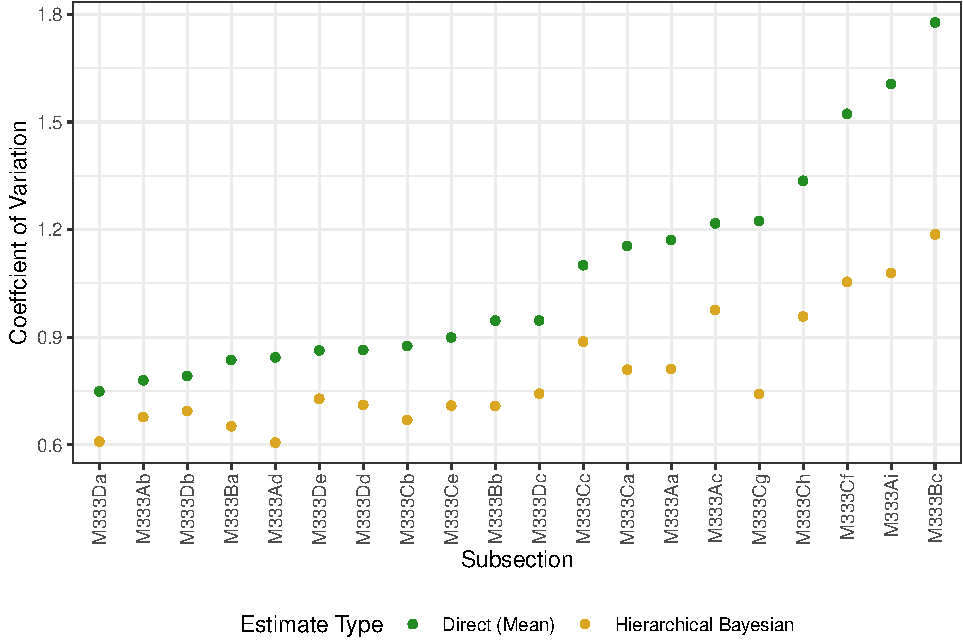
\includegraphics[width=0.9\linewidth]{thesis_files/figure-latex/unnamed-chunk-18-1} 

}

\caption{Direct and model-based coefficients of variation for the unit-level model}\label{fig:unnamed-chunk-18}
\end{figure}
We see reductions in every coefficient of variation from the direct estimator to our model-based approach, with an average reduction in of 24.17\%. However, the variation we see is still much larger than wanted, with the ecosubsection with the lowest coefficent of variation just over 0.6 and the overall coefficient of variation of the model at a value of 0.76. These large coefficients of variation indicate that even though we were able to reduce the variance in the estimate by an average of 24.17\%, the will not perform well enough to be used as a reliable predictor of average biomass.

\hypertarget{discussion-and-conclusion}{%
\chapter{Discussion and Conclusion}\label{discussion-and-conclusion}}

If we don't want Conclusion to have a chapter number next to it, we can add the \texttt{\{-\}} attribute.

\textbf{More info}

And here's some other random info: the first paragraph after a chapter title or section head \emph{shouldn't be} indented, because indents are to tell the reader that you're starting a new paragraph. Since that's obvious after a chapter or section title, proper typesetting doesn't add an indent there.

\appendix

\hypertarget{the-first-appendix}{%
\chapter{The First Appendix}\label{the-first-appendix}}

This first appendix includes all of the R chunks of code that were hidden throughout the document (using the \texttt{include\ =\ FALSE} chunk tag) to help with readibility and/or setup.

\textbf{In the main Rmd file}
\begin{Shaded}
\begin{Highlighting}[]
\CommentTok{# This chunk ensures that the thesisdown package is}
\CommentTok{# installed and loaded. This thesisdown package includes}
\CommentTok{# the template files for the thesis.}
\ControlFlowTok{if}\NormalTok{ (}\OperatorTok{!}\KeywordTok{require}\NormalTok{(remotes)) \{}
  \ControlFlowTok{if}\NormalTok{ (params}\OperatorTok{$}\StringTok{`}\DataTypeTok{Install needed packages for \{thesisdown\}}\StringTok{`}\NormalTok{) \{}
    \KeywordTok{install.packages}\NormalTok{(}\StringTok{"remotes"}\NormalTok{, }\DataTypeTok{repos =} \StringTok{"https://cran.rstudio.com"}\NormalTok{)}
\NormalTok{  \} }\ControlFlowTok{else}\NormalTok{ \{}
    \KeywordTok{stop}\NormalTok{(}
      \KeywordTok{paste}\NormalTok{(}\StringTok{'You need to run install.packages("remotes")",}
\StringTok{            "first in the Console.'}\NormalTok{)}
\NormalTok{    )}
\NormalTok{  \}}
\NormalTok{\}}
\ControlFlowTok{if}\NormalTok{ (}\OperatorTok{!}\KeywordTok{require}\NormalTok{(thesisdown)) \{}
  \ControlFlowTok{if}\NormalTok{ (params}\OperatorTok{$}\StringTok{`}\DataTypeTok{Install needed packages for \{thesisdown\}}\StringTok{`}\NormalTok{) \{}
\NormalTok{    remotes}\OperatorTok{::}\KeywordTok{install_github}\NormalTok{(}\StringTok{"ismayc/thesisdown"}\NormalTok{)}
\NormalTok{  \} }\ControlFlowTok{else}\NormalTok{ \{}
    \KeywordTok{stop}\NormalTok{(}
      \KeywordTok{paste}\NormalTok{(}
        \StringTok{"You need to run"}\NormalTok{,}
        \StringTok{'remotes::install_github("ismayc/thesisdown")'}\NormalTok{,}
        \StringTok{"first in the Console."}
\NormalTok{      )}
\NormalTok{    )}
\NormalTok{  \}}
\NormalTok{\}}
\KeywordTok{library}\NormalTok{(thesisdown)}
\CommentTok{# Set how wide the R output will go}
\KeywordTok{options}\NormalTok{(}\DataTypeTok{width =} \DecValTok{70}\NormalTok{)}
\end{Highlighting}
\end{Shaded}
\textbf{In Chapter \ref{ref-labels}:}

\hypertarget{the-second-appendix-for-fun}{%
\chapter{The Second Appendix, for Fun}\label{the-second-appendix-for-fun}}

\backmatter

\hypertarget{references}{%
\chapter*{References}\label{references}}
\addcontentsline{toc}{chapter}{References}

\markboth{References}{References}

\noindent

\setlength{\parindent}{-0.20in}
\setlength{\leftskip}{0.20in}
\setlength{\parskip}{8pt}

\hypertarget{refs}{}
\leavevmode\hypertarget{ref-whatisfia}{}%
FIA. (2020). Forest inventory and analysis national program. \emph{What is FIA?} Retrieved from \url{https://www.fia.fs.fed.us/about/about_us/}

\leavevmode\hypertarget{ref-nlcd11}{}%
Homer, C. (2015, November). Completion of the 2011 national land cover database for the conterminous united states -- representing a decade of land cover change information. \emph{EPA}. Environmental Protection Agency. Retrieved from \url{https://cfpub.epa.gov/si/si_public_record_report.cfm?Lab=NERL\&dirEntryId=309950}

\leavevmode\hypertarget{ref-mcconville2020}{}%
McConville, K. S., Moisen, G. G., \& Frescino, T. S. (2020). A tutorial on model-assisted estimation with application to forest inventory. \emph{Forests}, \emph{11}(2), 244.

\leavevmode\hypertarget{ref-ver2017}{}%
Ver Planck, N. R., Finley, A. O., \& Huff, E. S. (2017). Hierarchical bayesian models for small area estimation of county-level private forest landowner population. \emph{Canadian Journal of Forest Research}, \emph{47}(12), 1577--1589.


% Index?

\end{document}
